\documentclass[10pt,a4paper]{article}
\usepackage[utf8]{inputenc}
\usepackage{amsmath}
\usepackage{amsfonts}
\usepackage{amssymb}
\usepackage{amsthm}

\usepackage{float}
\usepackage{subfigure}
\usepackage{framed}
\usepackage{xcolor}

\usepackage{graphicx}
\graphicspath{{images/}}

\definecolor{shadecolor}{gray}{0.9}

\newtheorem{questions}{Question}
\newenvironment{question}
   {\begin{shaded}\begin{questions}}
   {\end{questions}\end{shaded}}

\author{Ram\'on Mart\'inez}
\title{BCPNN and Sequence Learning}

\begin{document}
\maketitle

\section{Introduction}

\cite{lashley1951problem}

\section{The BCPNN as a Sequence Learner}


\begin{figure}[h!]
\centering
\includegraphics[scale=0.50]{ampa2.pdf}
\caption{The network posses a wide dynamical range}
\end{figure}

\begin{align*}
\tau_m \dfrac{s_i}{dt} &= \beta_i + \sum_{j} w_{ij} o_j + a_i - s_i \\
o &= \frac{exp(s_i)}{\sum_j exp(s_j)} \\
\tau_z \dfrac{dz_i}{dt} &= o_{i, k} - z_{i} \\
\tau_p \dfrac{dp_i}{dt} &= z_i(t) - p_i(t)  \\  
\tau_p \dfrac{dp_{ij}}{dt} &= z_i(t) z_j(t) - p_{ij}(t)\\
w_{ij} &= \log(\frac{p_{ij}}{p_i p_j}) \\
\beta_i &= \log(p_i) 
\end{align*}




\bibliographystyle{unsrt}
\bibliography{references.bib}

\end{document}





